\section{创建 Date 类}
\hfill\ctli{实验时间}{~2015~年~1~月~8~日}
\subsection*{【实验目的】}
\begin{enumerate}[topsep=0pt,partopsep=0pt,itemsep=0pt,parsep=0pt,label={\arabic*、}]
\item 掌握创建类的方法。
\item 熟悉成员函数的使用方法。
\item 掌握函数和指针的概念
\item 掌握函数和指针的使用方法。
\end{enumerate}
\subsection*{【实验环境】}
\MyEnvironment
\subsection*{【实验内容】}
\begin{enumerate}[topsep=0pt,partopsep=0pt,itemsep=0pt,parsep=0pt,label={\arabic*、}]
\item P89:3.15
\item P348:8.12
\item P354:8.20
\end{enumerate}

\subsection{Date 类}
\subsubsection*{【详细分析】}
创建一个名为 Date 的类,包括了作为数据成员的三部分信息:年月日,都为 int 类型。包括一个具有三个参数的构造函数,用以初始化年月日。假定给出的年、日是正确的,对于不在 1--12 的月,默认设置为 1。对每个数据成员都提供 set/get 函数。提供 displayDate 功能显示格式化后的日期。
\subsubsection*{【实验源码】}
{\linespread{1}\lstinputlisting[caption={\tt Date.h}]{exp04/Date.h}}
{\linespread{1}\lstinputlisting[caption={\tt Date.cpp}]{exp04/Date.cpp}}
{\linespread{1}\lstinputlisting[caption={\tt exp01.cpp}]{exp04/exp01.cpp}}
\subsubsection*{【实验结果】}
\begin{figure}[htp]
\centering
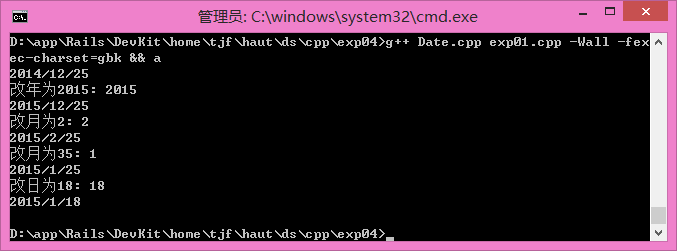
\includegraphics[width=\textwidth]{exp04/exp01.png}
\caption{\label{out04_01}Date 类}
\end{figure}

\subsection{P348:8.12}
\subsubsection*{【详细分析】}
修改课本上的程序,使发牌函数发一手 5 张牌,完成任务:
\begin{enumerate}[topsep=0pt,partopsep=0pt,itemsep=0pt,parsep=0pt,label={\alph*)}]
\item 确定手上是否有一对牌
\item 确定手上是否有两对牌
\item 确定手上是否有 3 张同号牌
\item 确定手上是否有 4 张同号牌
\item 确定手上是否有同花
\item 确定手上是否有顺子
\end{enumerate}

程序对花色和点数分别进行累计,然后循环数出数量。
\subsubsection*{【实验源码】}
{\linespread{1}\lstinputlisting[caption={\tt DeckOfCards.h}]{exp04/DeckOfCards.h}}
{\linespread{1}\lstinputlisting[caption={\tt DeckOfCards.cpp}]{exp04/DeckOfCards.cpp}}
{\linespread{1}\lstinputlisting[caption={\tt exp02.cpp}]{exp04/exp02.cpp}}
\subsubsection*{【实验结果】}
\begin{figure}[htp]
\centering
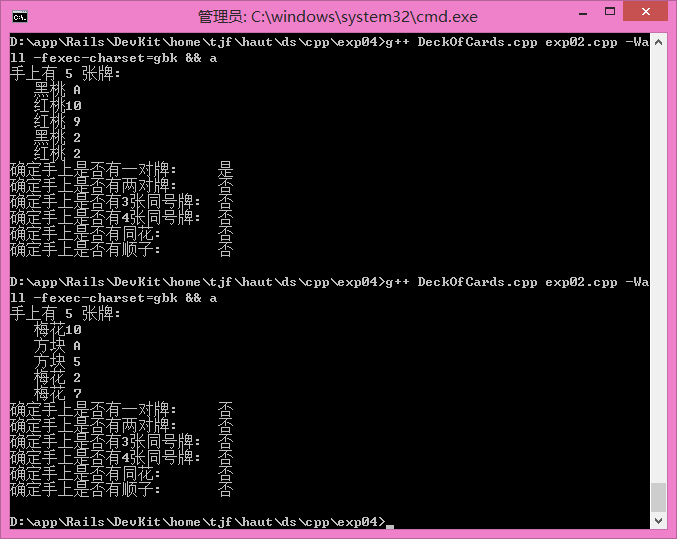
\includegraphics[width=\textwidth]{exp04/exp02.png}
\caption{\label{out04_02}发牌和判断程序}
\end{figure}

\subsection{P354:8.20}
\subsubsection*{【详细分析】}
修改洗牌和发牌程序,使之由同一个函数实现。
\subsubsection*{【实验源码】}
{\linespread{1}\lstinputlisting[caption={\tt DeckOfCards\_plus.cpp}]{exp04/DeckOfCards_plus.cpp}}
{\linespread{1}\lstinputlisting[caption={\tt exp03.cpp}]{exp04/exp03.cpp}}
\subsubsection*{【实验结果】}
\begin{figure}[htp]
\centering
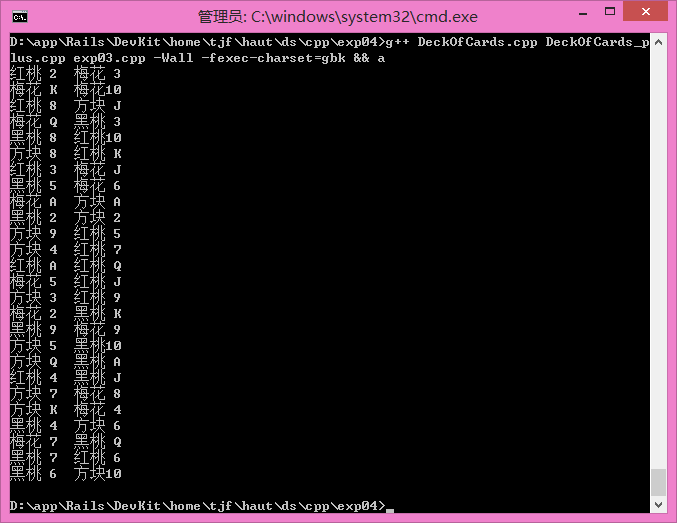
\includegraphics[width=\textwidth]{exp04/exp03.png}
\caption{\label{out04_03}发牌程序}
\end{figure}


\subsection*{【实验体会】}
这次的实验是 Date 类的简单实现,以及对 DeckOfCards 类的修改和增添功能。

对于初始化函数,也就是构造函数,可能会用冒号句法来简化成员对象的赋值。这里因为涉及到特殊判断,所以调用了三个设置函数,而对设置值的特殊处理则分别在设置函数中实现。访问函数有 const 属性,直接返回其值,并不改变值的大小。

判断发牌的花色和点数,则使用了循环查找的暴力算法,由于花色 $n = 4$, 点数 $m = 13$,那么 $O(n)$ 和 $O(m)$ 的算法实际上可以算作常数级别的了。为了简化查找,增设了两个数组来存储花色和点数。函数具有一定的通用性。

最后一个程序删掉了本来的注释,程序显得简练很多了。
